\begin{savequote}[75mm]
Some Quote.
\qauthor{Quoteauthor Lastname}
\end{savequote}

%For an example of a full page figure, see Fig.~\ref{fig:myFullPageFigure}.

\chapter{Tracking Based Point Cloud Video Segmentation}
\label{Chap:TrackingBasedSegmentation}
\newthought{There's something to be said} for having a good opening line. 

\section{Tracked Model Representation}
While ideally one could directly track supervoxels themselves, this is generally not reliable due to the aperture problem seen in neural visual fields~\cite{MarrApertureProblem}; local motion can only be estimated perpendicular to a contour that extends beyond its field of view~\cite{shimojo1989}. This means that in order to properly estimate motion of supervoxels, we must extend our considered field of view significantly beyond the size of the supervoxel itself; in fact, our aperture must contain the borders of the object, otherwise pairwise association of supervoxels is indeterminate. 

As such, we first merge supervoxels into contiguous higher level object groupings. For this work, we use a plane fitting and removal algorithm to remove supporting surfaces, followed by a euclidean clustering of the remaining supervoxels as in \cite{Radu3dIsHere}. It should be stressed that the overall tracking itself is independent of the segmentation used to initialize objects; one could easily use a model-based segmentation, or even a 2D classifier scheme on the original RGB image. Regardless of the segmentation used, the supervoxel clusters found are used to initialize the models which will be tracked.

\section{Supervoxel-Based Particle Filters}
Tracking of the segmented models is accomplished using a bank of independent parallel particle filters. The models consist of clouds of supervoxels, and observations are the supervoxels produced using the persistent scheme discussed in Section~\ref{sec:Supervoxels}. The observation model measures distance in a feature space of spatial distance, normals, color (in HSV space), and labels. Weights of predicted states ( $x,y,z$, roll, pitch, yaw) are measured by associating observed supervoxels with nearest supervoxels from the transformed models, and then measuring total distance in the feature space as (\ref{eqn:PFCoherence}). That is, the weight $w^k_i$ of particle $i$ belonging to object $k$ (of size $N_k$) with state $x_i$ is the sum of the products of the coherences $W$,
\begin{equation}
\label{eqn:PFCoherence}
w^k_{i} \sum_{p,q \in x_i} W_d W_{HSV} W_n W_l ~~.
\end{equation}
Coherences are calculated for each correspondence pair between model supervoxel $p$ and observed supervoxel $q$,
\begin{equation}
\label{eqn:DistTerms}
 \begin{array}{lcl}
 W_d & = & \frac{1}{1 + \frac{ \| p - q \|^2}{3 {R}_{seed}^{2}}} \\
 W_{HSV} & = & \frac{1}{1 + \|p_{HS}-q_{HS}\|^2} \\
 W_n & = & \frac{1}{ 1 + \left| 1 - n_p \cdot n_q \right| } \\
 W_l & = & \begin{cases} 1, & L_p = L_q \\ 
                         \frac{N_k-1}{N_k}, & L_p \neq L_q 
           \end{cases} 
 \end{array} ,
\end{equation}

where supervoxel $q$ has label $L_q$, normal $n_q$, and hue \& saturation $p_{HS}$.

KLD sampling \cite{KLDParticleFilter} is used to dynamically adapt the number of particles to the certainty of predictions. As matching supervoxel labels gives a high certainty of a correct prediction, objects which are not moving, and therefore have static supervoxel labels, need very few particles for accurate tracking. Details of the particle filters themselves are beyond the scope of this work, but we refer the reader to \cite{KLDParticleFilter} for an in-depth description of their operation. For this work, it is sufficient to understand that the particle filters yield independent predictions of 6DoF object state, allowing a transformation of the model to the current time-step - roughly aligning it with the currently observed supervoxels.  

\section{Association by Joint Energy Minimization}
The final step in the tracking process is to associate the observed supervoxels to the predictions coming from the particle filters, that is, we need to solve the multiple target data association problem. This is accomplished using an energy minimization which seeks to find an optimal global association of supervoxels to predictions. To do this, we first create a list of all observed supervoxels which lie within a radius $R_{seed}$ of each predicted supervoxel coming from the particle filters (see Fig.~\ref{fig:Association}). Then we determine all supervoxels which could only be associated with one possible object, associate them, and remove them from further consideration.

\begin{figure}[tb]
  \centering
  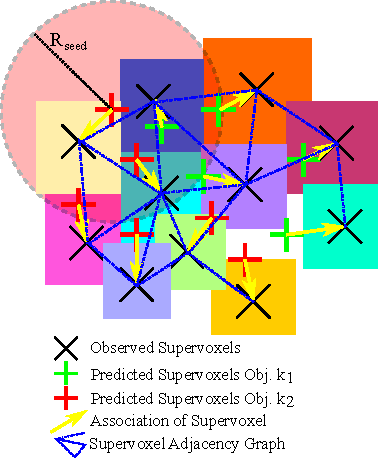
\includegraphics[scale=1.0]{figures/IROS2013/Association.pdf}
  \caption[Supervoxel Association]{Association of observed supervoxels with predicted model supervoxels using global energy.}
  \label{fig:Association}
\end{figure}

To associate the remaining observed supervoxels, we determine which objects are competing for them, and then find the predicted supervoxel from each object which lies closest to them in the feature space (using spatial location, normals, and color as in (\ref{eqn:Distance})). We adopt a RANSAC-like approach, similar to \cite{EnergyBasedMultiModel}, to sample from the set of possible associations and determine a global association which best aligns the predictions to the observed supervoxels. Additionally, we use a weighted sampling strategy where the likelihood of assigning object $k$ as the label $L$ of supervoxel $q$ falls off with increasing distance from the object centroid $C_k$
\begin{equation}
 \label{eqn:WeightSampling}
 \mathcal{L}(L_q=k | C_k) = \frac{1}{C_k}.
\end{equation}

To score a set of assignments, we compute a global energy, given in~(\ref{eqn:Energy}). Each global label association $\mathcal{A}$ consists of local associations $a$ which assign an object label $k$ to each observed supervoxel $q$. The first summation term, $ \sum_{p}{\|p_k - q\|} $, measures error in feature space between the observed supervoxel and the closest supervoxel in its associated predicted object $p_k$. 

\begin{equation}
\label{eqn:Energy}
{E}_\mathcal{A} =\prod_{a\in\mathcal{A}}{\Delta_k} \left( \sum_{p}{\|p_k - q\|} + \lambda \sum_{(q,q')\in \mathcal{N} }\delta(L_q \not= L_{q'}) \right) 
\end{equation}

The second summation is a smoothing prior which considers the adjacency graph of observed supervoxels. For every observed supervoxel, we compare its assigned label $L_q$ to the label of all supervoxels $q'$ which lie within its adjacency neighborhood $\mathcal{N}$. We adopt the Potts model as in \cite{Boykov2001}, where $\delta(\dot)$ is 1 if the specified condition holds, and 0 otherwise, and $\lambda$ is a weighting coefficient which controls the importance given to spatial continuity of labels.

Finally, the multiplicative term $\prod_{a\in\mathcal{A}}{\Delta_k}$ controls for the expansion or contraction of object volumes through the number of observed supervoxels associated with them. $\Delta_k$ penalizes for changes in volume by increasing the energy for deviations from unity in the ratio of observed supervoxels assigned to an object $\hat{N}_k$ with the number in the object model itself $\hat{N}_k$, that is

\begin{equation}
\label{eqn:DeltaSVs}
\Delta_k = \left\{ 
  \begin{array}{l l}
    {\hat{N}_k}/{N_k} & \quad \text{if ${\hat{N}_k} \geq {{N}_k}$ }\\
    2 - {\hat{N}_k}/{N_k} & \quad \text{if $\hat{N}_k < {N}_k$}~. 
  \end{array} \right.  
\end{equation}

Once the energy arrives at a stable minimum, we extract the resulting association of observed supervoxels to predicted results, and use them to update the tracked models.

\begin{figure*}[!ht]
  \centering
  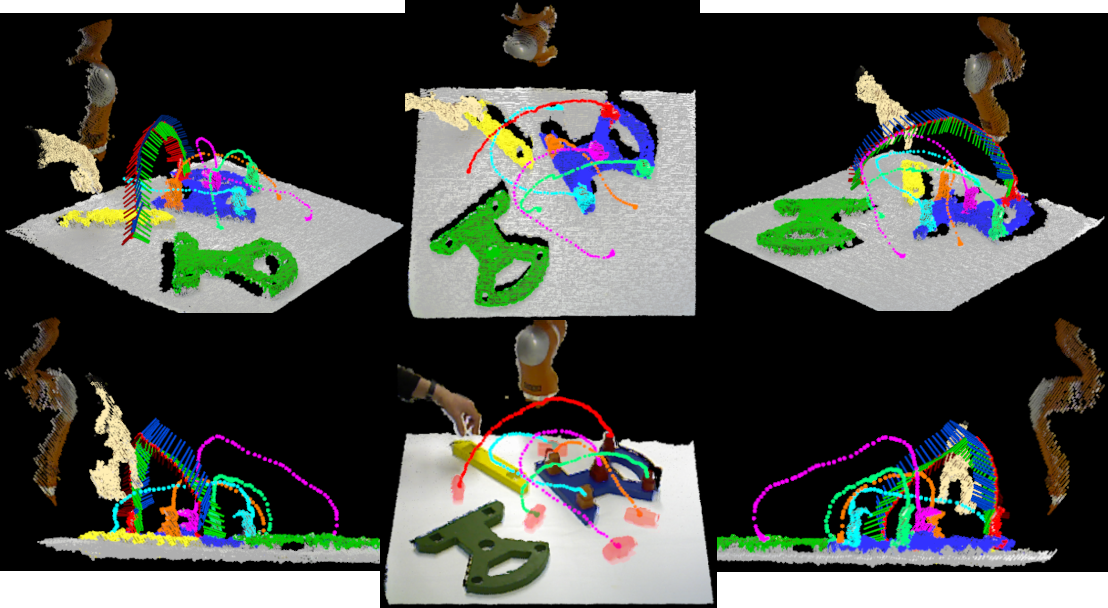
\includegraphics[width=\linewidth]{figures/IROS2013/TrajectoriesNew.pdf}
  \caption[Cranfield Tracking Results]{Result of tracking and segmentation on Cranfield scenario from different views. Here the tracks are shown as dots of the color of the tracked label for each timestep. Initial locations of the pegs are shown in the middle bottom frame as semi-transparent masks. Calculated orientation is shown for the red peg with a set of axes every second time-step; these axes show pose in a frame relative to the start. }
  \label{fig:Trajectories}
\end{figure*}

\section{Alignment and Update of Models}
The joint energy minimization results in a global association $\mathcal{A}$ which assigns observed supervoxels to tracked objects. In order to use this to update the object models, we determine a transform which aligns it to the internal representation stored by the particle filter. As an initial guess, we use the inverse of the predicted state, and then use an iterative closest point \cite{ICPChetverikov} procedure to refine the transform such that the set of observed supervoxels best aligns with the model prior. We then replace the model prior with the new observed supervoxels. 

As a final step, we use the refined transform to update the states of the particles. To do this, we shift each particle $x_i$ towards the refined state $\hat{x}$, weighting the importance given to the refined state by a constant factor $\epsilon$

\begin{equation}
\label{eqn:PFUpdate}
x'_{i \in L} = (1-\epsilon) x_i + \epsilon \hat{x}~.
\end{equation}

For this work, we found that an $\epsilon$ of $0.5$ effectively removes noise (jitter) introduced by the replacement of the tracked model. Additionally, we correct the internal motion model of the particle filters to correspond to the new updated state.

\section{Occlusion Handling}
\section{Experimental Results}
In order to demonstrate the usefulness of the proposed method, in this Section we provide results from two successful applications. Both applications use the Cranfield scenario \cite{collins1984development}, a benchmark developed for assessing performance of assembly robot systems. Fig.~\ref{fig:Trajectories} and the supplementary material\footnote{See also http://www.youtube.com/watch?v=0dVzWgW6Bs8 and https://www.youtube.com/watch?v=GjmUhm2JitU for longer versions.} show the results of tracking and segmentation (only the pegs are shown in Fig.~\ref{fig:Trajectories} to avoid clutter) using our Cranfield pieces. It can be seen that the algorithm is able to successfully track 6DoF states through the whole assembly task, even maintaining proper tracks for the pieces when they are fully occluded.

%%%%%%%%%%%%%%%%%%%%%%%%%%%%%%%%%%%%
\subsection{Imitation of Trajectories for Robot Manipulation}
\begin{figure}[!tb]
  \centering
  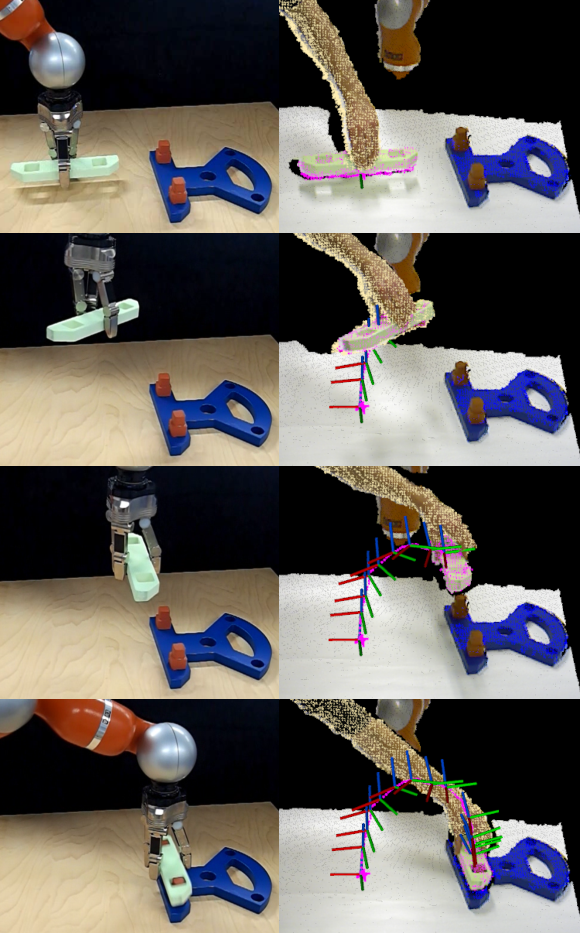
\includegraphics[scale=0.84]{figures/IROS2013/RobotImitation.pdf}
  \caption[Trajectory Imitation]{Kuka LWR arm imitating trajectory and pose learned from tracked human demonstration.}
  \label{fig:Imitation}
\end{figure}
The standard way of teaching robots to perform human-like actions is imitation learning, also called programming by demonstration \cite{Billard2008,Argall2009}. There are several ways to demonstrate movements: 1) recording movements in joint-space (joint angles) or target-space (Cartesian space) by ways of a motion capture device (requires putting markers on human body), 2) using kinaesthetic guidance (guiding a robot's movements by a human hand), or 3) via teleoperation (controlling a robot via joystick). The only way to obtain motion trajectories from human observation in a "non-invasive" procedure is by using stereo vision \cite{Hecht2009}, however, usually it is model based. The tracking algorithm we have presented here can be used as an alternative method to obtain motion trajectories (in Cartesian space) in a model-free way. 

To demonstrate this, we applied our tracking algorithm to obtain human motion trajectories in Cartesian space including orientation of manipulated object (in total six DoFs). We tested it using a recording of the Cranfield scenario where, first, we let a human demonstrate the action and then reproduced it using a KUKA Light Weight Robot (LWR) arm \cite{kuka}. Specifically, here we imitate a human putting the separator block on the pegs. To generate trajectories for the robot from human demonstrations, we used a modified version of Dynamic Movement Primitives \cite{Ijspeert2002,Ijspeert2013} (DMP) and learning method as described in \cite{Kulvicius2012}. We used Cartesian impedance control and, thus, generated six DMPs (three for motion of the end-effector in Cartesian space and three for orientation of the hand) based on trajectories obtained from the tracking algorithm. Here we used 100 equally spaced kernels with width $\sigma=0.05$ for each dimension (for more details please refer to \cite{Kulvicius2012}).
 As demonstrated in Fig.~\ref{fig:Imitation} and the supplementary video, trajectories obtained by the proposed tracking algorithm are sufficiently accurate to allow reproduction of the human motion.

%%%%%%%%%%%%%%%%%%%%%%%%%%%%%%%%%%%%

\subsection{Semantic Summaries of Actions}
A fundamental task for intelligent autonomous robots is the problem of encoding long chain manipulations in a generic way, for use in tasks such as learning and recognition. As a demonstration of the usefulness of the proposed tracking framework, we use a recently introduced novel Semantic Event Chain (SEC) approach \cite{Aksoy11} which converts each segmented scene to a graph: nodes represent segment (i.e. object) centers and edges indicate whether two objects touch each other or not. By using an exact graph matching technique the SEC framework discretizes the entire graph sequence into decisive main graphs. A new main graph is identified whenever a new node or edge is formed or an existing edge or node is deleted. Thus, each main graph represents a “key frame” in the manipulation sequence. Figure~\ref{fig:SECGraphs} shows a few detected sample key frames from the long Cranfield action. While the complete action has in total 1453 frames, the SEC representation reduces it to just 35 key frames, each of which 
represents a topological change in the scene.

\begin{figure*}[ht!]
  \centering
  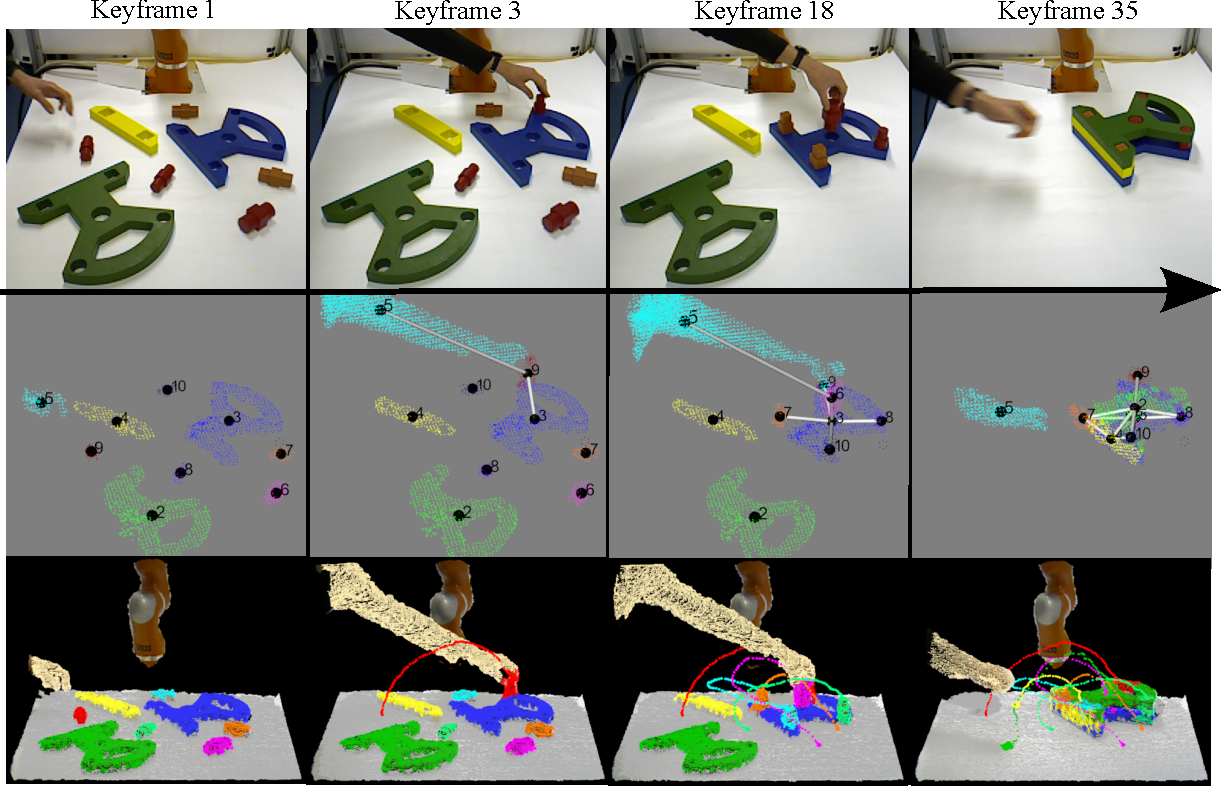
\includegraphics[width=\linewidth]{figures/IROS2013/SECKF.pdf}
  \caption[Cranfield Key Frames]{A few example key frames extracted from the long Cranfield action. Numbered nodes represent interacting objects, while edges show touching relations between objects. Each keyframe represents a topological change in the scene - here we show 4 of the 35 keyframes.}
  \label{fig:SECGraphs}
\end{figure*}



\section{Local Convex Patches}
\section{Hierarchy of Temporal Hypotheses}
\section{Hypothesis Pruning}
\section{Extracting a Realization of Perceptual Model}
\section{Experimental Results}

%\begin{figure}
%\includegraphics[width=\textwidth]{figures/fig1}
%\caption[Short figure name.]{This is a figure that floats inline and here is its caption.
%\label{fig:myInlineFigure}}
%\end{figure}



%% Requires fltpage2 package
%%
% \begin{FPfigure}
% \includegraphics[width=\textwidth]{figures/fullpage}
% \caption[Short figure name.]{This is a full page figure using the FPfigure command. It takes up the whole page and the caption appears on the preceding page. Its useful for large figures. Harvard's rules about full page figures are tricky, but you don't have to worry about it because we took care of it for you. For example, the full figure is supposed to have a title in the same style as the caption but without the actual caption. The caption is supposed to appear alone on the preceding page with no other text. You do't have to worry about any of that. We have modified the fltpage package to make it work. This is a lengthy caption and it clearly would not fit on the same page as the figure. Note that you should only use the FPfigure command in instances where the figure really is too large. If the figure is small enough to fit by the caption than it does not produce the desired effect. Good luck with your thesis. I have to keep writing this to make the caption really long. LaTex is a lot of fun. You will enjoy working with it. Good luck on your post doctoral life! I am looking forward to mine. \label{fig:myFullPageFigure}}
% \end{FPfigure}
% \afterpage{\clearpage}
